% !TeX root = ../main.tex

\chapter{石墨烯结构}


\section{石墨烯的结构}
\subsection{石墨的结构}
石墨为层状结构(图1),每一层中的6个碳原子构成平面网状结构,层和层之间以范德瓦尔斯力连接。\par
天然石墨一般有三种存在形式:无定形态、高结晶态、天然鳞片状。鳞片状石墨纯度较高,可达99$\%$,因更具有方向性,它比其它形式的石墨存在更大的研究价值和使用价值。\par
从C原子的堆积方式来看,石墨的C原子堆积方式主要有两种:一是以ABAB的顺序重复,具有六方晶系对称性,称为六方石墨;另一种结构是以ABCABC的顺序重复堆积,具有三方晶系对称性,称为三方石墨。六方石墨和三方石墨层间距离都为0. 335nm,层间作用力为范德瓦尔斯力。\par

{\begin{figure}[H]
        \centering
        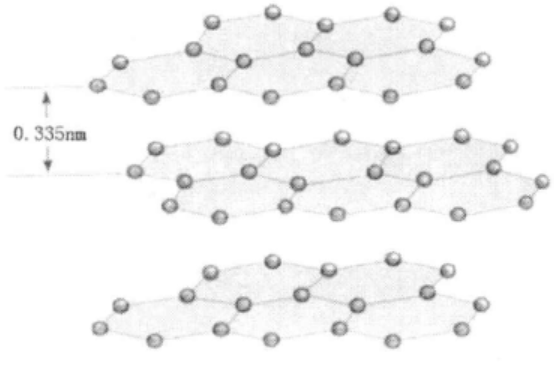
\includegraphics{img/石墨的结构图.png}
        \caption{石墨的结构图}
        \label{fig:my_label}
    \end{figure}}

\subsection{石墨烯的结构}
石墨烯是各种石墨结构的母体,是构建其它维数碳质材料的基本单元。二维石墨烯多层叠加形成三维的石墨体,卷曲可以形成一维结构的碳纳米管,包裹形成零维的球形富勒烯(图2)。所以这种最基础的结构是构筑其它材料的原型。\par
\begin{figure}[H]
    \centering
    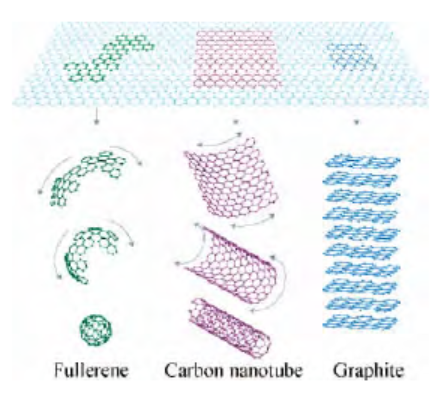
\includegraphics{img/石墨烯和几种炭材料的结构.png}
    \caption{石墨烯和几种炭材料的结构}
    \label{fig:my_label}
\end{figure}

单层石墨烯的厚度约$0.35nm$,碳-碳键长为$0.142nm$,理论上理想的单层石 墨烯的比表面积达$2630m^{2}/g$。\par
石墨烯中碳原子呈六环结构排列,这样独特的稳定结构使石墨烯具有较高的拉伸弹性模量($1TPa$)和抗拉强度($130GPa$)优良的导热性能、零带隙、电子-空穴迁移率高。当施加外部机械力时,碳原子层就会弯曲变形来适应外力,而不必使碳原子重新排列,这样就保持了结构的稳定。\par
石墨烯晶体结构中每个元胞包含两个碳原子,四个价电子的其中三个分别与邻近碳原子产生$sp^{2}$轨道杂化形成三个$\sigma$键,另外一个p轨道电子贡献给非局域化的$\pi$和$\pi^{*}$键,分别形成最高占据电子轨道和最低非占据电子轨道。而石墨烯的$\pi$和$\pi^{*}$键布里渊区K点处退化,费米面收缩成一个点,形成无带隙的金属能带结构(图3)。\par
\begin{figure}[H]
    \centering
    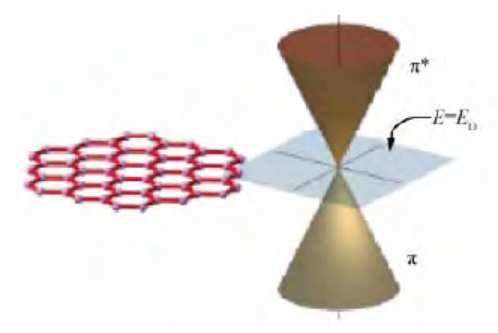
\includegraphics{img/单层石墨烯的电子结构.png}
    \caption{单层石墨烯的电子结构}
    \label{fig:my_label}
\end{figure}

\section{石墨烯的导电性及其应用}
\subsection{石墨烯的导电性}


我们可以依靠紧束缚模型计算出石墨烯的能带分布。在紧束缚模型中电子想要跃迁到其他地方,需要脱离原子的势场,所以我们将在一个原子附近的电子看作受该原子势场的作用为主,其他原子势场的作用看成微扰,从而可以得到能带分布。石墨烯的能带分布图如下。\par

\begin{figure}[H]
    \centering
    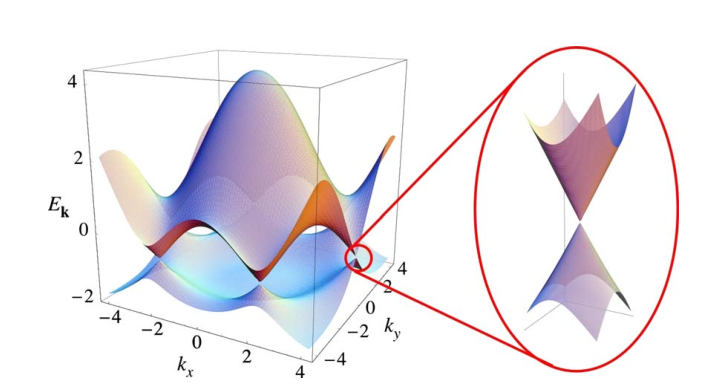
\includegraphics{img/石墨烯的能带分布,右边是狄拉克点附近.png}
    \caption{石墨烯的能带分布,右边是狄拉克点附近}
    \label{fig:my_label}
\end{figure}
在$K$,$K'$点附近,我们能得到附近波矢$k=K+q$的色散关系,$E_{\pm } (q)\approx \pm \frac{3ta}{2} \left | q \right | + O\left [(q/K)^{2}  \right ]$,是近似线性的。因此在量子力学中动量与波矢只差一个约化普朗克常量,因此动量与能量的关系为线性,因此电子的速度为常量,记$v_F=\frac{3ta}{2}$。\par
因为描述电子运动的时候,我们把一个在晶格内运动的电子等效为一个在自由空间中运动的电子,所以类似地引入有效质量的概念,将晶体中的场对于电子的影响等效于自由空间运动的电子的质量$\frac{1}{m_*}\sim \frac{d^{2}E}{dk^2}$,由于色散关系为线性,且在能量为零的点对称,导致$E(k)$在$K$点不连续,导致二阶导数无穷大,所以电子的有效质量为零。\par
故用薛定谔方程来描述粒子的运动已无效,应该运用引入了相对论效应的狄拉克方程来描述。事实上当我们将电子算符在$K$,$K’$进行傅里叶展开,代入哈密顿量之后,我们可以得到一个与二维的无质量电子的狄拉克方程近似的方程
\begin{equation}\label{...}
    iv_{F}\sigma \cdot \nabla \psi(r)=E \nabla (r)
\end{equation}
\par
波函数在$K$的分量为

\begin{figure}[H]
    \centering
    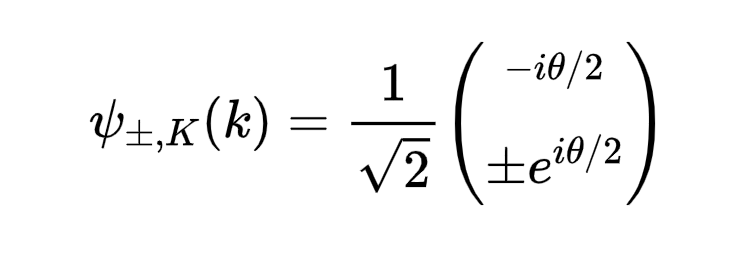
\includegraphics[width=0.20\textwidth]{img/EQ1.png}
\end{figure}
在$K'$的分量为
\begin{figure}[H]
    \centering
    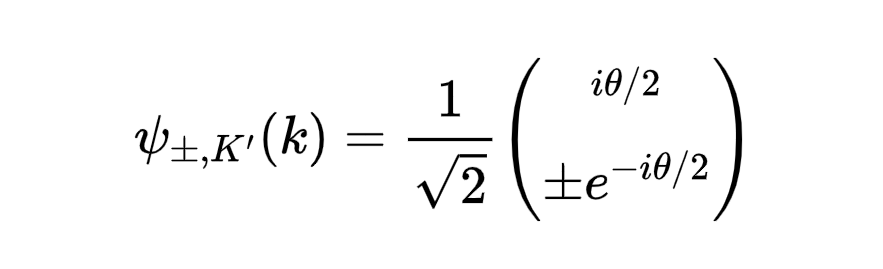
\includegraphics[width=0.20\textwidth]{img/EQ2.png}

\end{figure}
\par

将$M$作为原点,两个分量的方向轴对称,且相位差为$\pi$,粒子波函数在两个波矢方向的分量可以等效为一组自旋量。螺旋度是动量算子对于自旋方向的投影,螺旋度的算子定义为$\hat{h} =\frac{1}{2} \sigma \cdot \frac{p}{\left | p \right | }  $。由于自旋量是粒子的波函数的动量分量,所以其螺旋度为$\pm 1/2$。这与狄拉克方程中所描述的无质量的自旋为$\pm 1/2$的电子相似,狄拉克方程中,正离子自旋方向只会与动量方向相同,反粒子自旋方向与动量方向相反,而在石墨烯中$K$,$K'$附近的电子就对应的是正粒子,空穴对应的是反粒子。这样电子与空穴与狄拉克方程所描述自由空间中无质量的两种状态的电子等效,所以我们可以把石墨烯狄拉克的空穴与电子称为狄拉克费米子,$K$,$K'$被称为狄拉克点。\par
空穴与电子也可以在能量为零的点相互转化,且不消耗能量,因此若改变石墨烯纵向的电压,可以得到不同种类和浓度的载流子,这也就是我们可以制造石墨烯场效应管的原因。\par
关于石墨烯非常高的电子迁移率的原因也是由于狄拉克点的存在,由于量子隧穿效应的影响,电子有概率穿过高于自身能量的势场,对于如下图的势场,通过计算我们可以得到狄拉克费米子的隧穿概率:
\begin{equation}\label{...}
    T(\phi )\simeq \frac{cos^{2}\phi }{1-cos^{2}(Dq_{x})sin^{2} \phi }
\end{equation}
\par
$\phi$趋于$0$时概率趋于$1$,这是石墨烯和狄拉克费米子特别的性质。这意味着石墨烯中的电子和空穴有较长的自由程,电子运动受温度影响较小。石墨烯有很高的电子迁移率。\par
以上说明石墨烯有良好的导电性。\par



\subsection{石墨烯导电性的应用}
\subsubsection{超级电容器}
超级电容器是是介于电容器和电池之间的储能器件,是传递能量和储存能量的体系。石墨烯的比表面积非常大而且导电性能优异,使得电子的聚集能力提高且扫面电压稳定。使用石墨烯作为电极大大减少了充电时间而且容量提高了$5-6$倍。\par
\begin{figure}[H]
    \centering
    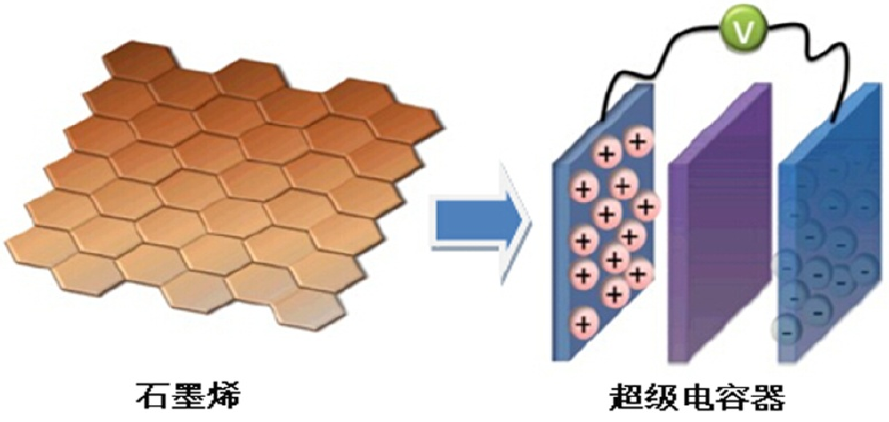
\includegraphics{img/石墨烯用于超级电容器的电极材料.png}
    \caption{石墨烯用于超级电容器的电极材料}
    \label{fig:my_label}
\end{figure}
Stoller等人使用单层石墨烯作为超级电容器的电极,分别在水中比电容为$135F/g$ 和在有机电解液中比电容为$99F/g$。Le等人使用的新的方法将石墨烯溶液直接喷墨打印在钛网上,然后通过热还原法制备出石墨烯薄膜的超级电容器。经过伏安法扫描$1000 $次后,比电容从$ 125F/g $下降到$121F/g$,损失率不到 $3\%$。Ning 等人用模板化学沉积法制备可控结构的石墨烯网,石墨烯网厚度有 $1-2$ 层,比表面积有$1654m^{2}/g$。将石墨烯网作为超级电容器电极在KOH 溶液中测试比电容达到$245F/g$ 同时 $2000$ 次伏安循环后还保持在 $94.1\%$。制备的基于石墨烯的平面结构的超级电容器,质量比电容可以达到$250F/g$,面积比电容高于以前的报道达到了$394F/cm^{2}$。\par
基于石墨烯的超级电容器方面具有非常大的应用潜力。目前就提高石墨烯比表面积和导电性,还有较大的突破空间。\cite{ref1} \par

\subsubsection{石墨烯在锂离子电池中的应用}
石墨烯因具有巨大的比表面积、优异的电性能和稳定的化学性能,目前已被广泛应用于锂离子电池的负极材料中。锂离子电池的负极主要作为储锂的主体,石墨烯既具备提供良好电子传输通道的能力,又有优异的锂离子传输性能,故能提升传输性能。Yoo等采用氧化还原法制备得到石墨烯,并将其应用于锂离子电池负极材料,实验数据显示,首次循环的比容量有明显提升,比容量值可达$540 mAh/g$。\par
石墨烯在二维高比表面积上具备特殊结构,因此被应用于锂离子电池的正极材料中。该项特点使电子的传输能力得到进一步提升,从而对正极材料的导电性能进行全面改善,并提升了锂离子的传输能力。目前的研究表明,石墨烯与LiFePO$_{4}$、LiNi$_{1/3}$Co$_{1/3}$Mn$_{1/3}$O$_{2}$和LiMn$_{2}$O$_{4}$等复合形成的复合正极材料可提升材料的电化学性能。\cite{ref2} \par

\subsubsection{石墨烯在防腐涂料的应用}
石墨烯薄膜能贴附在金属表面,将金属与氧气、水等隔绝,加入到原有的涂料中,使得涂料表面的空隙减小,加强隔绝性能;石墨烯机械性能良好,掺入防腐涂料后形成迷宫状结构,具有优异的弹性和抗变形能力;石墨烯具有优良导电性,可以采用电化学防腐。故石墨烯在防腐涂料领域广泛应用。 \par
石墨烯在防腐涂料的应用分为石墨烯薄膜、石墨烯功能化修饰、石墨烯填料。
石墨烯薄膜很难被腐蚀,能够对被贴附的材料进行有效的保护,例如石墨烯掺杂量为$0.4\%$时,能够将聚酰胺涂层的摩擦寿命提高$880\%$。功能化修饰例如以乙二胺与氧化石墨烯表面的羧基发生脱水缩合反应,制得纳米氧化石墨烯(NGO,Nano Graphene Oxide)。之后以NGO作为填料,加入到环氧树脂涂料中,制备得到复合防腐涂料。以石墨烯做环氧树脂涂料的填料可以有效地增强环氧树脂涂料的耐腐蚀能力、力学性能,延长使用寿命。\cite{ref4} \par

\section{石墨烯的其他性质及应用}
\subsection{石墨烯的其他性质}
石墨烯片具有超高的力学强度,这是由于极强的碳碳键相互作用。石墨烯的杨氏模量有$1TPa$\cite{ref5},断裂强度达$130GPa$,断裂强度超过普通钢材强度的$200$多倍\cite{ref6},是目前力学强度最高的材料。\par
石墨烯也具有优秀的导热性。在室温条件下其热导率为$(5.3±0.48)×103 W/m \cdot K$,最高可达到$6000 W/m \cdot K$\cite{ref7},明显高于纳米级碳纳米管的导热率$(3500  W/m \cdot K)$。石墨烯也是目前热导率最好的材料。
石墨烯的表面积大,且透明。单层石墨烯片的表面积为$2630m^{2}$g。且经过红外光谱的分析发现单层石墨烯仅有少量的光吸收,透光率达$97.7\%$ \cite{ref8,ref9},几乎完全透明。
化学性质上,由于碳碳键组成的石墨烯在性质上与苯环相似,然而石墨烯是由多个六元环组成导致了许多性质又有所不同。从宏观上看,石墨是由许多多层的石墨烯叠加而成,使得石墨烯同时具有稠环的部分性质和石墨的化学性质。\par

\subsection{石墨烯的其他应用}
\subsubsection{石墨烯新型吸附剂}
石墨烯、氧化石墨烯以其层絮状结构、优异特性及其功能化改性等特征可作为新型吸附剂材料,在环境水体和土壤中污染的修复、大气污染治理等方面具有较大的应用潜力。例如石墨烯/碳(G/C)复合气凝胶可以吸附水中污染物土霉素、布洛芬;\cite{ref10}聚合离子液体修饰的氧化石墨烯吸附剂能够用于工业废水等水体中去除亚甲基蓝的新型吸附剂\cite{ref11}。\par
\subsubsection{石墨烯储氢}
石墨烯储氢即石墨烯虽然可以隔绝所有气体和液体,却能够对质子“网开一面”。科学家设计出的“三明治结构”将碳氮材料夹在两层石墨烯中,然后再利用光能产生激子,这些光能产生的激子分离后会形成正负电荷,并分别分布于外层石墨烯和碳氮“夹心”层。\par
石墨烯表面的水分子在正电荷的帮助下分解,产生质子。这些质子可穿透石墨烯,并在遇到电子后发生反应,进而产生氢气。由于只有质子能够通过石墨烯,而产生的氢气不能穿透石墨烯,所以光解水产生的氢气分子会被安全地保留在“三明治结构”内。同时氧原子、氧气、羟基等物质无法进入复合体系,从而抑制了氧与氢重新变为水的逆反应发生,实现了高储氢率下的安全储氢。\par
石墨烯对氢气的极强的吸附能力可以引入到氢能源汽车及飞机等交通工具领域,将带来良好的经济、环境、社会效益。\par
\subsubsection{氧化石墨烯抑菌性及应用}
氧化石墨烯(GO)是含氧官能团分布在表面及边缘上,并伴有部分缺陷位点的单层石墨烯。2010年上海应用物理所樊春海课题组以GO为抗菌剂,对革兰氏阴性大肠杆菌的杀菌效果进行研究,结果表明,浓度为$85\mu g/mL$的GO经过2h的接触时间后能够几乎完全抑制大肠杆菌的生长,抑菌率达$98.5\%$。\cite{ref12}\par
目前关于GO抗菌性能有三种主流机理,分别为来自GO纳米级锋利的边缘的膜穿刺,活性氧(ROS)依赖或非依赖引起的氧化应激作用,以及GO柔性薄膜结构对细菌的缠绕或捕获。\par
利用GO的抑菌性,可以明显抑制大肠杆菌的滋生,龋病、牙周炎及种植体周围炎主要致病菌如链球菌、牙龈卟啉单胞菌、具核梭杆菌等,这对人体细胞是无害的。\par

\section{结束语}
自石墨烯成功制备以来,其在科学界造成了巨大反响。石墨烯是一种低维材料,具有优良的导电性、光电子特性、特殊的量子隧穿效应、超导特性、理论上存在的量子反常霍尔效应,以及特殊的力学、热学与化学性质。随着其制备方式的不断改进和工业化发展,这些性质逐步得到工业上的广泛应用,并逐渐展现出广阔的市场前景,一点一滴地改变着我们的生活。\par



